\subsection{Routage}

Nous avons vu comment les machines obtenaient leurs adresses, de quoi étaient constitués les
paquets IPv4 et comment elles pouvaient communiquer entre elles.  Nous avons
donc maintenant des réseaux constitués d'une ou plusieurs machines, mais ces
réseaux sont indépendants et totalement hermétiques les uns des autres. Il
pourrait être intéressant de pouvoir faire communiquer ces réseaux entre eux.
C'est le but du routage que de faire passer des paquets d'un réseau à un autre.

\subsubsection{Principe du routage}

\paragraph{Materiel}
Le routage est une action qui va être déléguée à une machine servant à établir
un lien entre deux ou plusieurs réseaux.  Le matériel qui va s'occuper de faire
cela est appelé un routeur: cela peut être n'importe quel ordinateur configuré
pour faire du routage, ou dans la plupart des cas une machine "dédiée", celle-ci
étant conçu pour le routage et ayant des caractéristiques adaptée à cette tache
(nombre des interfaces réseaux, consommation réduite, accélération matérielle, ... ).

Comme un routeur se charge de faire les liaison entre différents réseaux, il doit
forcément avoir deux ou plusieurs interfaces réseaux: au moins une pour chaque
réseau qu'il doit lier.

\paragraph{Table de routage}
Afin que le routeur puisse envoyer un paquet vers sa destination, il faut qu'il
sache vers quelle direction transmettre le paquet pour qu'il soit sur le bon
réseau. Il faut pour cela qu'il ait une table regroupant les associations entre
les réseaux et la direction vers laquelle ils se trouvent: cette table est
appelée table de routage.  Cette table de routage peut être remplie de plusieurs
manières: soit manuellement par l'administrateur réseau (le réseau est donc
figé et n'est pas tolérant aux pannes), soit dynamiquement à l'aide de
protocoles de routage (RIP, OSPF, BGP, IS-IS,...) qui vont modifier en temps
réel la table de routage pour s'adapter aux changements du réseau et être
tolérant aux pannes.

Lorsque les hôtes d'un réseau ont besoins de contacter un autre réseau par le
biais d'un routeur, ils vont également utiliser une table de routage.  En
effet, lorsqu'un hôte veut envoyer un paquet vers un autre réseau, il faut
qu'il ait l'adresse du routeur auquel envoyer son paquet pour que celui-ci le
transmette en direction du bon réseau.

\paragraph{Forwarding}

Lorsqu'un routeur reçoit un paquet qui ne lui est pas destiné il va utiliser
l'entré de sa table la plus précise pour joindre le réseau de destination.

Pour faire cela il essaye de déterminer quel NET ID de sa table de routage
correspond le mieux à l'adresse de destination.  Une fois trouvée, il va transmettre
le paquet vers la direction associée à celui-ci.
Cette direction peut être:
\begin{itemize}
\item Soit être une interface: dans ce cas le réseau en question se trouve
directement derrière cette interface. Il faut donc envoyer le paquet
directement à son destinataire.
\item Soit une adresse IP: qui désigne l'adresse du prochain routeur auquel il
faut envoyer le paquet et qui va s'occuper à son tour de diriger le paquet vers
sa destination.
\end{itemize}

\subsubsection{Routage en IPv4}
\paragraph{Agrégation CIDR}
L'adressage avec masque CIDR a permit de réduire la taille de la table de
routage en agrégeant plusieurs entrées en une seule; ce qui était impossible avec
l'utilisation de classes d'adresses.  En effet, avec les classes d'adresses, le
masque étant fixé et les classes ne se chevauchant pas, il n'était pas
possible de créer une hiérarchie entre les réseaux.  Ainsi il n'est pas
possible d'agréger plusieurs réseaux en une seule entrée dans la table de
routage.

\begin{figure}[h]
\centering
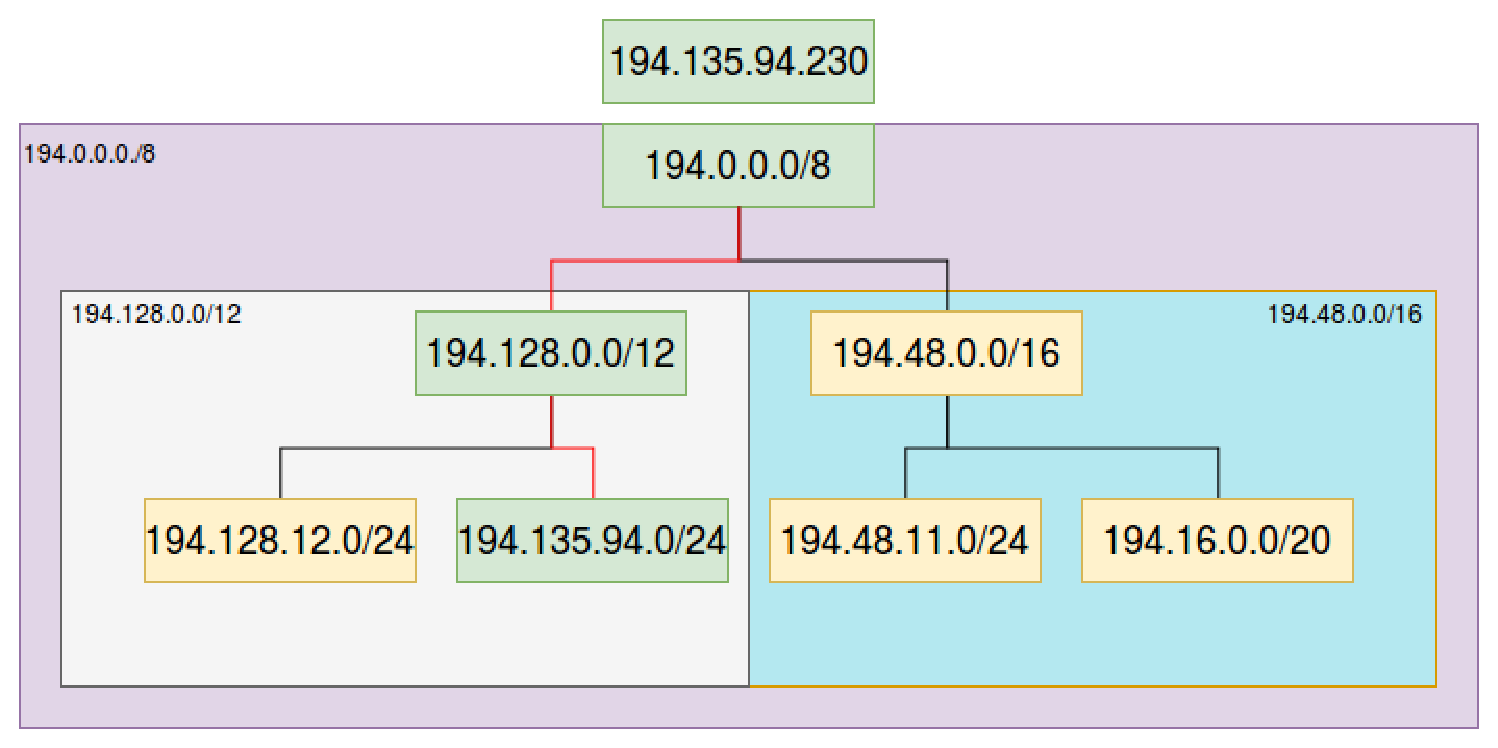
\includegraphics[width=15cm]{./pics/routagecidr.eps}
\caption{Agregation des adresses reseau base sur leur hierarchie}
\label{fig:routcidr}
\end{figure}

L'adressage avec un masque CIDR permet d'être totalement libre dans le choix du
masque. Ceci permet de créer une hiérarchie entre les réseaux. De ce fait,
un routeur n'est pas obligé de créer une entrée pour chaque réseaux dans la
table de routage mais, quand il est possible, il créera seulement une entrée
comme étant l'agrégation des réseaux sous-jacents représentés par l'entrée.



\paragraph{Adresses spéciales}


Comme nous l'avons vu plus haut, certaines adresses sont utilisées pour des
tâches particulières. Cela peut induire un traitement particulier lors du routage
d'un paquet.  C'est le cas par exemple des adresses de {\it lien local} qui ne
peuvent jamais traverser un routeur pour joindre un réseau différent. En effet
les adresses de lien local sont propres à un réseau.
Un autre cas où les adresses sont limitées est le cas des adresses de broadcast.
En temps normal, les routeurs bloques les paquets émis en broadcast, de sorte qu'ils ne se propagent pas en dehors du réseau d'origine. Il est facile d'imaginer les problèmes que causerait un paquet émit en broadcast sur Internet. Une exception étant les paquets DHCP émient en broadcast et qui traversent les routeurs par le biais des agents DHCP.
Un dernier cas particulier constitue les adresses privées: le routage des paquets ayant une adresse privée en destination n'a pas de sens en dehors d'un réseau privé. Les adresse privées peuvent passer les routeurs et avoir du sens du moment qu'elle reste dans un réseau privé.

